% !TEX root = ../../prj4projektdokumentation.tex


\section{Trinskifter}
\label{sec:Trinskifter}
For at kunne skifte trin og dermed spændingsniveau på transformeren er der opbygget et kredsløb med tre kontaktrelæer - et for hvert muligt trin. Det er et krav, at relæerne skal kunne styres både automatisk og manuelt fra en PLC. Udgangssignalet fra PLC'en er 24VDC,så dette skal relæerne altså kunne holde til. På værkstedet var kun en type relæ der kan holde til 24VDC styresignal, og derfor faldt valget på disse Hengstler 468 relæer, se bilag B4 for datablad. På figuren nedenfor ses tegning af relækredsløbet samt de forskellige belastninger, der kan kobles ind via kontakter. I serie med hver belastningsmodstand sidder en 1 $\Omega$ modstand, som måleenheden måler over. 


\begin{figure}[H] 
	\centering
	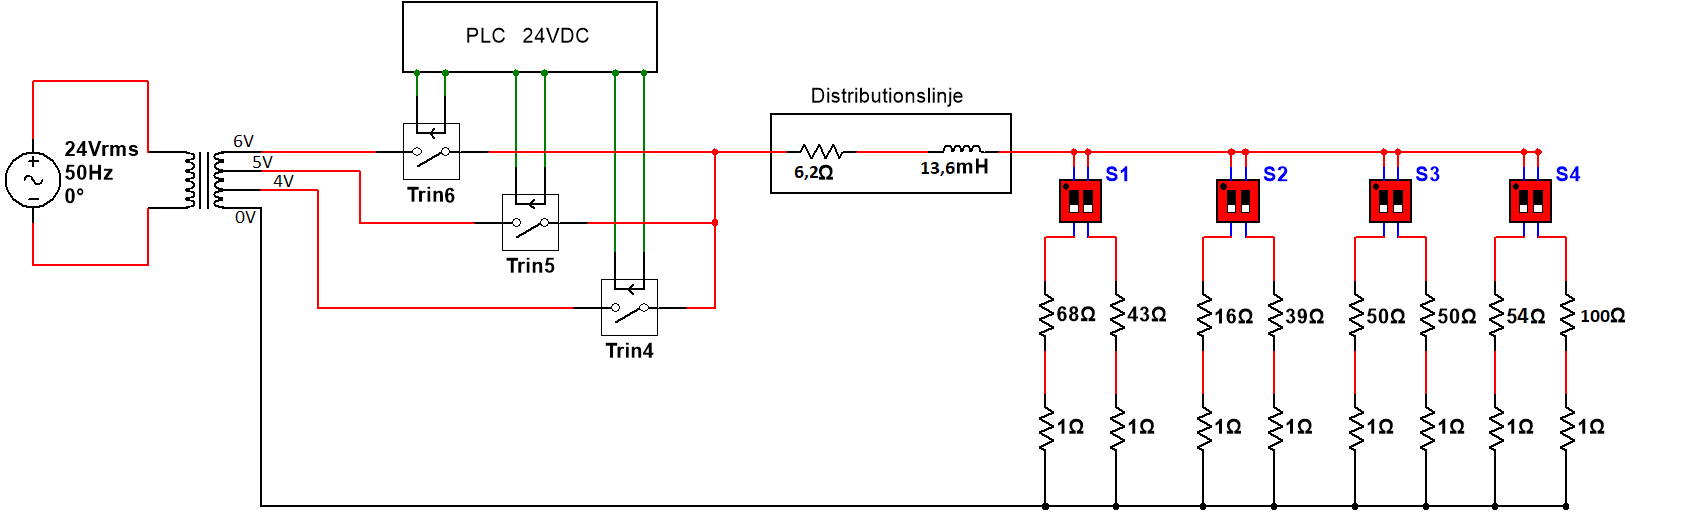
\includegraphics[width=1\textwidth]{Figure/Trinskiftertegning2}
	\caption{Kredsløbstegning af Distributionslinje, belastninger og Trinskifter}
	\label{fig:Trinskiftertegning2}
\end{figure}

Som vist på tegningen er hver relæspole forbundet til hver sin udgang på PLC, og det er herfra de modtager styresignalet. Hvert relæ er desuden forbundet til henholdsvis trin 4, 5 og 6. Gennem en Normally Open contact i hvert relæ er trinene videre forbundet ud til distributionslinjen. Ved skift af trin fra eksempelvis 4 til 5 sendes højt signal til begge trin og herefter slukkes signalet til trin 4. Der er altså et overlap ved skift af trin, og på den måde forsvinder forsyningen til belastningen ikke undervejs. 

Relækredsløbet er implementeret på et printkort, der forbindes til transformertrinene via bananstik, og til PLC og distributionslinje via pins. Det færdige kredsløb ses på figur \ref{fig:Relaekredsloeb}

\begin{figure}[H] 
	\centering
	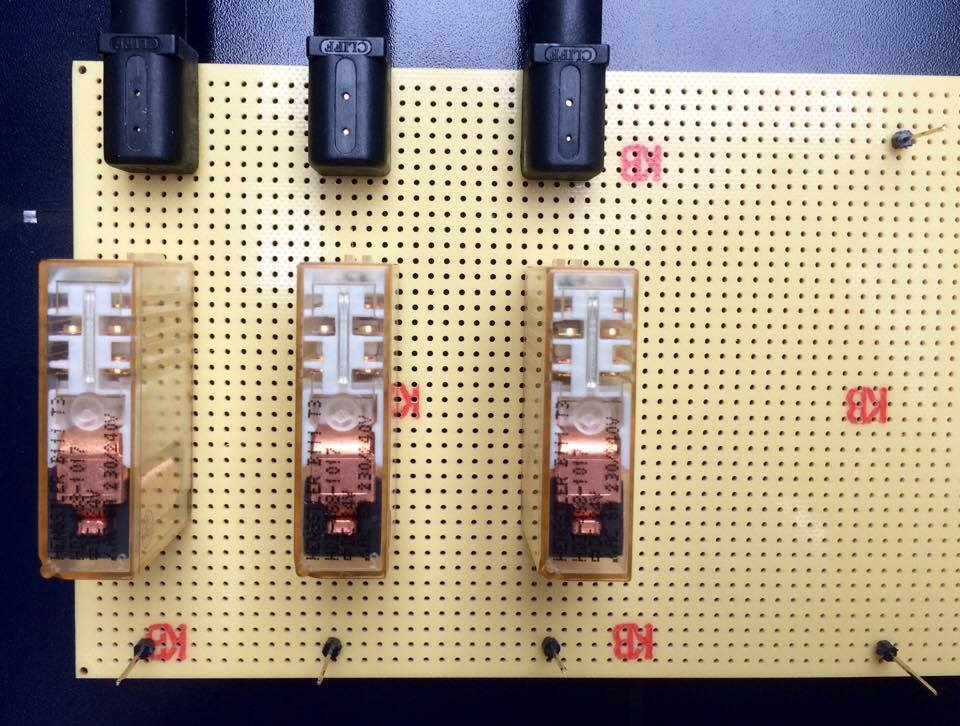
\includegraphics[width=0.8\textwidth]{Figure/Relaekredsl}
	\caption{Relæer på printkort}
	\label{fig:Relaekredsloeb}
\end{figure}

